\chapter{Trusted Platform Modules}\label{tpm}
Il \textbf{TPM} (\textit{Trusted Platform Module}) è un chip hardware progettato per ottenere livelli di sicurezza migliori rispetto a quanto offrono le soluzioni puramente software. Offre servizi di crittografia, memoria sicura, calcolo e monitoraggio dell’integrità della piattaforma. È in realtà un componente versatile, poiché dopo la specifica 2.0 nasce anche il \textbf{TSS} (\textit{TPM Software Stack}), ovvero un’\textbf{API} (\textit{Application Programming Interface}) che permette alle applicazioni di accedere ad alcune primitive di sicurezza offerte dal TPM stesso.

\section{Storia}

\subsection{Cosa viene prima della soluzione TPM?}
Prima di poter parlare di TPM, è utile affrontare un diverso concetto di soluzione per il problema dell’hardware sicuro. 
Un \textbf{HSM} (\textit{Hardware Security Module}) è un dispositivo fisico o una rete di dispositivi con il compito di proteggere, gestire e scambiare chiavi digitali, oltre che svolgere alcune operazioni crittografiche dedicate (come il calcolo hash per le firme digitali). Gli HSM incarnano un’idea un po’ più generale ed astratta di piattaforma affidata rispetto al TPM.

L'HSM e il TPM sono entrambi dispositivi hardware progettati per garantire la sicurezza hardware delle chiavi, dei dati e del codice riservato, ma hanno anche un'altra similarità: permettono di ottenere l’isolamento delle operazioni crittografiche in un ambiente controllato, così da ridurre i rischi di intercettazione e manipolazione. 

La differenza principale, però, è rappresentata dal fatto che gli HSM tradizionali offrono una sicurezza più robusta e con maggiori prestazioni; inoltre, sono utilizzati in ambienti distribuiti, data center e applicazioni complesse e di alto livello. Gli standard che un HSM deve rispettare (anche per fini governativi e finanziari) sono molto più rigorosi rispetto a quanto stabilito per i TPM montati sui \textbf{PC} (\textit{Personal Computer}) del cittadino privato medio.
I TPM sono più piccoli e, nella maggior parte dei casi, integrati direttamente nei dispositivi consumer di cui si vuole garantire protezione e integrità. 

Tra gli obiettivi della specifica del \textbf{TCG} (\textit{Trusted Computing Group}) -- il consorzio che realizza le specifiche TPM -- non c’era il raggiungimento di particolari velocità d’esecuzione, per questo motivo i TPM non sono degli acceleratori crittografici. Questa specifica non si prende l’impegno di fornire strumenti che puntino a ottimizzare ed efficientare l'utilizzo delle risorse in sé, bensì si prefigge di fornire strumenti e servizi.
Non è una \textit{secure enclave} perché non prevede la possibilità di eseguire codice, ma tramite altre funzioni riesce a verificare firme digitali sul software o la sua integrità -- quindi può verificare l’affidabilità del codice.

In sintesi, il TPM è una forma di HSM, una soluzione ad una parte del problema che quest’ultimo vuole affrontare, ma calato nell’ambiente locale e adattato specificamente per i dispositivi consumer.

\subsection{Perché nasce il TPM?}
A partire dal 2003 la tecnologia legata al TPM viene sviluppata secondo le specifiche del TCG, per poi iniziare a essere distribuita su larga scala.
Lo storico delle versioni comincia nel 2003: la specifica 1.1b metteva nero su bianco per la prima volta le funzioni base di un TPM, ma portava con sé diverse criticità. Per questo motivo tra il 2005 e il 2011 viene sviluppata la versione 1.2, poi migliorata ulteriormente nel 2014 con la 2.0.

L'introduzione di questa tecnologia ha segnato un passo significativo nell'evoluzione delle soluzioni per la protezione dei dati, mettendo a disposizione quei dispositivi hardware in grado di garantire integrità e autenticazione che si ricercavano sin dall’inizio degli anni ’90. L’adozione del TPM ha trovato spazio in ambiti che vanno dalla protezione di dispositivi personali alla gestione di informazioni sensibili, come quelle trattate da entità governative e da organizzazioni che gestiscono dati segreti o altamente riservati.

\subsection{Il Trusted Computing Group}
Le principali aziende del settore PC si sono quindi unite e hanno iniziato a lavorare ad un nuovo approccio hardware e allo sviluppo di uno standard industriale. Nel 1999 nasce la \textit{Trusted Computing Platform Alliance}, con l’obiettivo di creare \textit{Trusted Clients} (dispositivi personali) per rendere le applicazioni importanti come reti, comunicazioni ed e-commerce più sicure.

Parallelamente si ambiva ad uno standard aperto e con diffusione quanto più capillare possibile per informare il pubblico tecnico in tempo utile e creare fiducia. Lo standard del \textit{Trusted Computing} si basa in gran parte sull'esperienza acquisita tra gli anni ’90 e 2000 con le \textit{smart card} ad alta sicurezza e le loro applicazioni.

Il TCG ricevette forti pressioni sui costi, dunque qualsiasi soluzione avessero progettato doveva essere a basso impatto economico per il consumatore finale -- ad esempio facendo in modo che il modulo hardware aumentasse il costo di un PC di un dollaro o meno, per consentirne una diffusione capillare. In sintesi, il TPM nasce perché serviva una forma di HSM specificamente adattata per dispositivi personali. Il risultato fu un chip hardware passivo destinato ad essere fisicamente collegato alla scheda madre di un PC.

Il set di comandi TPM fu progettato per fornire tutte le funzioni essenziali per i suoi casi d'uso di sicurezza; tutto ciò che non era assolutamente necessario veniva spostato dal chip al software. Il TPM ha come obiettivo proteggere i dati utente e i processi critici tramite un ambiente sicuro e di garantire l'integrità della piattaforma. Lo standard descrive come utilizzare i meccanismi crittografici per ottenere queste funzionalità. Attraverso le indicazioni del TCG, il TPM fornisce l'autenticazione e l'accreditamento della piattaforma, non dell'utente.

\clearpage
\subsection{HRoT secondo il TCG}
Secondo il TCG, un \textbf{HRoT} (\textit{Hardware Root of Trust}) è un componente di sicurezza fondamentale che fornisce funzioni affidabili per l’intero sistema, costituendo la base sulla quale si fondano tutti gli altri meccanismi di fiducia. Questi componenti sono progettati per avviare una catena di fiducia che assicura l'integrità del sistema, impedendo che venga eseguito codice dannoso. 

Il TPM rappresenta una delle implementazioni più comuni di un HRoT, soprattutto per dispositivi come computer e laptop. Il TPM è progettato per raccogliere informazioni sul processo di avvio e monitorare se il sistema è nello stato previsto, garantendo autenticazione e integrità attraverso l'uso di chiavi sicure. 
Per ambienti virtualizzati, è stato sviluppato anche un \textbf{vTPM} (\textit{virtual TPM}), che replica le funzioni di un TPM fisico attraverso il software, garantendo comunque l'affidabilità richiesta per l'attestazione e la generazione di chiavi. Quest’ultimo non è un HRoT, ma solo un \textbf{RoT} (\textit{Root of Trust}), non essendo fisicamente un componente a sé stante.

Nel contesto di una piattaforma affidabile basata su TPM, il TCG definisce tre componenti logici essenziali che formano la HRoT:
\begin{itemize}
    \item \textbf{Root of Trust for Storage (RTS):} si occupa della protezione e archiviazione sicura di dati sensibili, come chiavi private, attraverso meccanismi di cifratura simmetrica e asimmetrica. Utilizzando operazioni di \textit{seal} e \textit{unseal}, il TPM gestisce questi dati in modo sicuro senza che siano mai direttamente memorizzati all'interno del chipset, ma piuttosto in memoria centrale cifrata.
    \item \textbf{Root of Trust for Reporting (RTR):} questo componente è responsabile della misurazione e della verifica dell'integrità del sistema. Il TPM calcola gli \textit{hash digest} dei vari componenti del sistema e li firma digitalmente per garantire la loro autenticità. Ciò permette di monitorare l’integrità complessiva della piattaforma, creando una tracciabilità sicura.
    \item \textbf{Root of Trust for Measurement (RTM):} il RTM è un meccanismo che esamina e verifica l'integrità della piattaforma durante il processo di avvio. Gestito dal \textbf{CRTM} (\textit{Core Root of Trust for Measurement}), il RTM misura lo stato del sistema e assicura che non vi siano stati compromessi, utilizzando componenti come il \textit{BIOS boot block} o la tecnologia \textit{Trusted Execution} di Intel.
\end{itemize}

Il TPM integra i concetti di RoT attraverso una struttura di sicurezza che include componenti hardware e software. Questi componenti logici di RoT -- RTS, RTR e RTM -- svolgono ruoli cruciali nel mantenimento dell'integrità del sistema, proteggendo sia i dati che le operazioni eseguite, e costituiscono la base della fiducia della piattaforma.

È interessante osservare come il concetto di RoT venga, invece, definito dal forum \textbf{UEFI} (\textit{Unified Extensible Firmware Interface}): si cita un \textit{“hardware-validated boot process to ensure the system can only be started using code from an immutable source”}. La differenza sostanziale sta nella parola “componente” contro “\textit{hardware-validated}”, implicando che le implementazioni della specifica TCG possano essere realizzate anche virtualmente, simulate o tramite puro software.

\clearpage
\section{La specifica 1.2}
La specifica del TPM originale comprendeva già le funzioni base di un TPM, purtroppo però portava con sé diverse criticità. Il TPM realizzato secondo la specifica 1.1b non era immune agli attacchi a dizionario e non prevedeva nemmeno un’interfaccia standard a livello hardware. Questo si tradusse nella necessità di realizzare e utilizzare driver diversi in base al \textit{pinout} dei circuiti utilizzati dai singoli produttori. 

Nel 2011 viene diffusa la specifica 1.2, che comunque supportava solo l’algoritmo \textbf{SHA-1} (\textit{Secure Hash Algorithm 1}) per il calcolo hash. Purtroppo dal 2014 SHA-1 non è più considerato sicuro rispetto ad attacchi \textit{brute force}, motivo per cui oggi questa versione della specifica è completamente deprecata e inutile dal punto di vista della sicurezza.

La specifica del TPM venne progettata per essere indipendente dall’hardware, con l'idea che sarebbe stato necessario scrivere ulteriori documenti solo qualora si fosse cercata l'implementazione su una particolare piattaforma. 
Anche se il PC è la piattaforma su cui i TPM sono maggiormente distribuiti, il TCG ha gruppi di lavoro per piattaforme mobili, \textit{embedded} e virtualizzate. 

Nei PC, dalla versione 1.2, il TPM è solitamente implementato come un circuito integrato discreto in un pacchetto a piccolo contorno sottile da 28 pin. È collegato al bus \textbf{LPC} (\textit{Low Pin Count}) e può essere integrato in altri chip sulla scheda madre (ad esempio uno scanner di impronte digitali, un lettore di \textit{smart card}, un’entrata USB per caricare certificati digitali dall’esterno). Il firmware e il software del sistema operativo interagiscono con il TPM accedendo ai registri \textbf{PCR} (\textit{Platform Configuration Registers}) mappati in memoria e inviando comandi al chipset principale.

Ovviamente, per interagire con il chipset è necessario un livello software che sia in grado di accedere e attivare le funzionalità offerte dal TPM: esistono API open source, ma è anche possibile sviluppare \textit{custom software}. Questo tema verrà approfondito nel capitolo 4 (TPM Software Stack).

\subsection{Le funzionalità indicate da TCG}
Generalmente il TPM fornisce diverse funzionalità e strumenti alla sua piattaforma. Queste comprendono una serie di servizi di crittografia, autenticazione e integrità. I principali servizi offerti e gestiti da un TPM sono elencati di seguito.

\figura{0.6}{figures/architettura-tpm.png}{Architettura del TPM.}{fig:architettura_tpm}

Il \textit{secure storage} consente ai processi utente di cifrare i dati usando chiavi protette dal TPM (e note solo a quest’ultimo). Questo meccanismo permette di garantire che i dati sensibili siano sempre accessibili solo tramite TPM, riducendo il rischio di accesso non autorizzato.

La protezione delle chiavi consiste nel memorizzare in modo sicuro le varie classi di chiavi con cui il TPM lavora. Il metodo di accesso è selezionato in base al tipo di chiave (TPM-bound, migrabile, firma, identità o \textbf{AIK} [\textit{Attestation Identity Key}]): una chiave viene protetta maggiormente quanto più sono sensibili e critici i dati che difende.

La \textit{platform measurement and reporting} è il meccanismo che permette di verificare e comunicare l'integrità della piattaforma all’esterno. Tramite la generazione di report sulla configurazione della piattaforma, è possibile attestare l’affidabilità del sistema verso un’altra entità, basandosi su un’autorità terza come le \textbf{CA} (\textit{Certificate Authorities}). L’attestato di affidabilità di una piattaforma è sempre verificabile, e permettere che un’entità esterna possa farlo significa garantire la \textit{platform authentication}. 

I cambiamenti di stato o le modifiche alla configurazione della piattaforma sono memorizzati nei registri PCR, interni al TPM e protetti tramite l’hashing SHA-1.

Il TPM è anche un generatore di numeri casuali -- o \textit{nonce} -- tramite processi \textit{hardware-based}. Questa capacità sta alla base della generazione sicura e imprevedibile delle chiavi crittografiche, ma non solo.

Il \textit{file sealing} -- o solo \textit{Sealing} -- è il meccanismo che incapsula i dati sulla base di valori contenuti nel PCR. In altre parole, il TPM associa dei dati alla configurazione della piattaforma (trovata nel PCR) e poi li firma con il valore hash della configurazione stessa. Il TPM decifrerà i dati se e solo se i valori nei PCR non sono stati alterati, quindi se la configurazione è quella attesa.

Nelle prossime sezioni verranno mostrate alcune delle funzionalità e capacità del TPM 1.2.

\subsection{Le chiavi principali}
I TPM hanno dei segreti detti \textit{seeds} (o semi) che non lasciano mai fisicamente il chip e non sono volatili. Sono usati per generare le chiavi e identificare il TPM stesso anche se la memoria esterna cambia o viene formattata. Dunque possiamo affermare che il TPM genera chiavi e le usa per dare informazioni di sé in modo attendibile ad entità terze. 

È importante sottolineare come uno dei punti principali delle Root of Trust (in questo caso incarnate dal TPM) sia fornire l’isolamento fisico dei segreti. Questo isolamento è essenziale sia per motivi di privacy, sia perché permette di proteggere le chiavi private anche quando il sistema operativo in esecuzione non è affidabile.

\subsubsection{Storage Root Key}
Nel TPM, le chiavi sono organizzate in una struttura ad albero e gestite in maniera gerarchica. Al vertice di questo albero c'è una chiave principale chiamata \textbf{SRK} (\textit{Storage Root Key}), che viene creata all'inizio del processo di inizializzazione del TPM. Questa chiave SRK è fondamentale perché permette di derivare tutte le altre chiavi, seguendo un modello gerarchico.

La SRK è generata e archiviata internamente al TPM e non viene mai esposta o spostata fisicamente all'esterno del chip.

\subsubsection*{Proprietà della Storage Root Key:}
\begin{itemize}
    \item Tutte le chiavi derivate sono protette dalla SRK. Questo significa che anche se una chiave derivata viene esportata dal TPM (ovvero trasmessa al di fuori del chip), rimane sempre cifrata dalla SRK.
    \item Poiché la SRK è unica per ogni TPM e non viene mai esposta, le chiavi derivate sono anche uniche: le chiavi figlie della SRK sono tutte e solo quelle cifrate -- o \textit{wrappate} -- dalla SRK stessa. 
\end{itemize}

Per ridurre i costi di produzione, il TPM ha la capacità di creare più chiavi a partire da un unico segreto. Il segreto è chiamato \textit{seed} e l'algoritmo utilizzato è detto \textbf{KDF} (\textit{Key Derivation Function}), ovvero funzione di derivazione della chiave. Il TPM può utilizzare le KDF per derivare sia chiavi simmetriche che asimmetriche.

Il TPM 1.2 opera con una singola autorizzazione del proprietario, utilizzando la SRK per la crittografia più esterna. Ogni chiave, che sia una chiave principale o figlia, è associata a un valore di \textit{authdata}, simile a una password, che autorizza il suo utilizzo. L'accesso a una chiave richiede la conoscenza di questo \textit{authdata} (per dimostrare di essere il proprietario della chiave), e i processi che desiderano utilizzare una chiave devono fornire la prova di questa conoscenza, ad esempio tramite un \textbf{HMAC} (\textit{Hash-based Message Authentication Code}). 

Il TPM tratta la conoscenza dell'\textit{authdata} come prova completa della proprietà dell'entità, senza la necessità di altri controlli. Il richiedente (qualsiasi entità che desideri eseguire un comando sul TPM o utilizzare una specifica entità) può avere protezioni e requisiti aggiuntivi dove salva l'\textit{authdata}; tuttavia, il TPM non impone ulteriori requisiti.

\subsubsection{Endorsement Key}
Esiste un’altra chiave (o meglio coppia di chiavi) detta \textbf{EK} (\textit{Endorsement Key}), sempre RSA a 2048 bit e sfruttata per le operazioni di firma e attestazione. 

Il TPM genera la EK prima che il cliente finale riceva la piattaforma. Il componente che causa la generazione della EK, chiamato \textbf{TPME} (\textit{Trusted Platform Module Entity}), è anche l'entità che creerà e firmerà il certificato EK, attestando la validità del TPM e della EK stessa. Il certificato permette di autenticare fortemente il TPM: l'Endorsement Key è un valore univoco per ogni TPM fisico.

Una volta che il TPM ha generato una prima EK, i tentativi successivi di generare o di inserire dall’esterno una EK devono fallire. Inoltre, la chiave deve esistere solo in memoria protetta -- interna al TPM -- e deve essere disponibile solo per entità autorizzate. Il TPME è tipicamente il produttore del chip TPM.

La Endorsement Key non può essere utilizzata per firmare digitalmente perché è progettata per essere utilizzata solo per autenticazione e identificazione. I motivi sono due:
\begin{enumerate}
    \item \textbf{Per la privacy:} la EK è una chiave che contiene informazioni sensibili legate al dispositivo. Questo potrebbe compromettere la privacy dell'utente o della piattaforma, poiché diventerebbe possibile risalire al dispositivo che ha firmato certi dati o autorizzato un’attività.
    \item \textbf{Per la sicurezza:} la EK è pensata per scenari di autenticazione, come l'attestazione dell'autenticità del TPM stesso. Se fosse utilizzata per firmare, ci sarebbe il rischio che la chiave privata venga esposta o utilizzata in modo improprio. Inoltre, una chiave di firma che viene utilizzata ripetutamente è più facilmente compromettibile rispetto a una chiave usata solo per autenticare.
\end{enumerate}

\subsubsection{Attestation Identity Keys}
Le \textit{Attestation Identity Keys} sono delle chiavi alias per la Endorsement Key. La EK viene utilizzata per generare l'\textbf{AIK} (\textit{Attestation Identity Key}), una chiave che è specificamente progettata per firmare, mentre la EK rimane confinata al suo ruolo di identificazione e attestazione.

Le AIK vengono usate principalmente per fornire un'autenticazione della piattaforma a un \textit{service provider} esterno, ma anche per proteggere l’integrità del firmware della piattaforma. Queste chiavi non firmano mai dei dati, bensì solo attestati o misurazioni. Il tipo di autenticazione che si ottiene tramite le AIK è approfondita nel paragrafo dedicato (Sezione \ref{subsec:daa}). 

Le AIK sono protette dalla SRK, che le cifra prima di spedirle all’esterno del TPM. Non è però corretto dire che le AIK derivano direttamente dalla SRK. Le AIK sono generate e certificate in un processo separato, principalmente utilizzando l'EK per garantire l'attestazione. L’unico legame con la SRK è per la loro protezione.

Dunque la EK può essere usata per dimostrare che un’AIK è stata generata da un TPM, senza però rivelare quale. Poiché il numero di AIK generabili è illimitato, è possibile distruggerle dopo l’uso o creare più AIK per scopi diversi (ad esempio, condividere informazioni diverse sulla piattaforma o l’utente con diverse entità). 

\subsection{Certificati}
Il TPM può conservare tre tipi di certificati fondamentali per garantire l'autenticità e la sicurezza della piattaforma: l'Endorsement Certificate, il Platform Certificate e il Conformance Certificate.
\begin{itemize}
    \item \textbf{Endorsement Certificate:} contiene la chiave pubblica della Endorsement Key e ha lo scopo di attestare che il TPM è autentico e che la sua EK è adeguatamente protetta. Questo certificato garantisce che il TPM proviene da una fonte affidabile ed è un componente sicuro per l'uso in applicazioni di \textit{Trusted Computing}. La fiducia associata ad un TPM deriva in gran parte dall’unicità della EK e dalla sua protezione costante. Anche per questo motivo le entità che generano la EK e quelle che rilasciano l'EC sono diverse, per evitare conflitti d’interesse.
    \item \textbf{Platform Certificate:} fornito dal produttore della piattaforma, conferma che i componenti di sicurezza della piattaforma stessa sono autentici e che un TPM valido è stato installato correttamente. Questo certificato viene utilizzato per stabilire fiducia nell'integrità della piattaforma hardware.
    \item \textbf{Conformance Certificate:} rilasciato dal produttore della piattaforma o da un laboratorio di valutazione accreditato, attesta che le proprietà di sicurezza della piattaforma sono state verificate e che essa è conforme agli standard stabiliti dal TCG. In sostanza, attesta che il chip TPM non è stato manomesso. 
\end{itemize}

Questi certificati consentono di stabilire con certezza l'autenticità di un dispositivo e la sua conformità agli standard di sicurezza, supportando meccanismi come la \textit{Direct Anonymous Attestation} per garantire un equilibrio tra verificabilità e anonimato. 

\subsection{Platform Configuration Registers}
All’interno del chip TPM esiste una struttura hardware che non rappresenta di per sé una funzionalità, ma diventa essenziale per garantire la correttezza di altre. Questa struttura si chiama \textbf{PCR} (\textit{Platform Configuration Registers}) ed è composta da registri \textit{special-purpose} interni al chipset TPM. I PCR sono impiegati in processi come il \textit{Secure Boot}, \textit{Measured Boot} e \textit{Remote Attestation} (o Attestazione Remota) per assicurare l’integrità e l'autenticità della piattaforma.

L’intuizione che porta alla progettazione di questa memoria viene accompagnata dalla necessità di avere registri per effettuare misurazioni alla sequenza di avvio di un sistema o al suo stato. La specifica definisce quale registro deve essere utilizzato per misurare ogni componente software coinvolto nel processo di avvio.

Questi registri sono della dimensione di un hash (20 byte, dettato da SHA-1 nel TPM 1.2) e non possono essere popolati con un certo valore direttamente, bensì è necessaria un'operazione intermedia: il software invia un comando di estensione al TPM specificando un numero PCR e un valore hash. 

Dal TPM 2.0 i registri hanno una dimensione variabile in funzione dell’algoritmo di hash configurato per il TPM: solitamente si impiega lo SHA-256, quindi saranno registri da 256 bit.

L’utilità di queste misurazioni è riscontrabile nella richiesta del TPM di garantire l’integrità del processo di avvio: memorizzare in maniera affidabile qualche misurazione di un software permette alla macchina di accorgersi quando si tenta di caricare del software non riconosciuto. “Non riconosciuto” significa non affidabile, ma non necessariamente! Potrebbe anche semplicemente trattarsi di un contenuto sviluppato indipendentemente da privati e senza passare attraverso le corporazioni che realizzano questi chip o loro affini, motivo per cui non viene riconosciuto.

\begin{figure}[htbp]
    \centering
    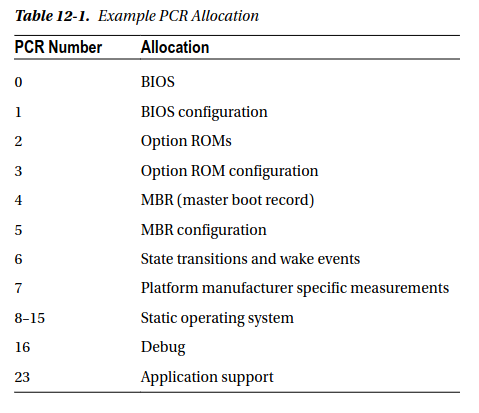
\includegraphics[width=0.8\textwidth]{figures/es-pcr.png} 
    \caption{Esempio di allocazione dei registri PCR.}\label{fig:allocazione_pcr}
\end{figure}

\subsection{Anonimizzazione delle chiavi (DAA)}\label{subsec:daa}
Da TPM 1.2 esiste anche il protocollo \textbf{DAA} (\textit{Direct Anonymous Attestation}), un meccanismo basato sul concetto di firme di gruppo. In questo schema, ogni entità coinvolta si fida e attesta reciprocamente l'autenticità delle altre, consentendo anche di dimostrare che una chiave è stata generata da un TPM senza rivelare né quale specifico TPM l'abbia creata, né informazioni a suo riguardo. 

La DAA rappresenta una forma di \textit{attestation} basata su metodi a \textit{zero knowledge} (\textit{direct proof}) e non necessita di una CA esterna, eliminando di fatto la necessità di un'entità terza esterna per la verifica. Questa funzionalità è particolarmente utile per stabilire se un sistema remoto con cui si sta comunicando è dotato di un TPM, senza esporre informazioni sensibili sull’identità del dispositivo.

La DAA sfrutta le chiavi AIK, descritte precedentemente. Il vantaggio di questo protocollo è che permette al creatore dell'AIK di scegliere una quantità variabile di informazioni che desidera trasmettere all’esterno, variando dall'anonimato perfetto (viene inviata la prova che un'AIK appartiene a un TPM, ma non quale) alla conoscenza perfetta (viene inviata la prova che una certa EK è associata a quella AIK). La differenza tra i due è evidente quando un TPM viene compromesso e la chiave privata di una particolare EK viene divulgata su Internet. A questo punto, una \textit{privacy CA} può revocare i certificati se sa che un certificato che ha creato è associato a quella particolare EK compromessa.

\subsection{Standardizzazione}
A partire dal TPM 1.2 il TCG decide di rendere la specifica TPM uno standard. Viene fornita un'interfaccia software standard e una configurazione dei pin del pacchetto più specifica rispetto alla 1.1b. Si mantiene comunque la compatibilità binaria del software per la versione 1.1b. 

\subsection{Attacchi a Dizionario}
Dopo il rilascio della 1.1b, il TCG si accorse immediatamente che il TPM non prevedeva alcuna resistenza agli attacchi a dizionario: non esistevano protezioni contro un aggressore che provava una password dopo l'altra nel tentativo di individuare quella corretta. La soluzione si individuò in maniera semplice, prevedendo un limite superiore ai tentativi di inserimento delle password per l’autorizzazione alla decifratura della chiave entro un certo intervallo temporale.

\subsection{NVRAM}
Durante lo sviluppo della specifica insorgono due punti problematici che richiedono un intervento progettuale:
\begin{enumerate}
    \item Il TPM è in grado di generare chiavi private, ma non dispone di memoria interna permanente per conservarle. Per ovviare a questa limitazione, può cifrare le chiavi con una chiave pubblica e archiviarle su disco, consentendo un recupero illimitato senza occupare spazio interno. Tuttavia, questo metodo diventa inapplicabile quando il sistema è spento, poiché, ad esempio, un disco crittografato non può contenere la propria chiave di decrittazione.
    \item Un'ulteriore criticità riguarda la gestione dei certificati di chiave di approvazione. Inizialmente, questi venivano memorizzati su disco, ma tale approccio si è rivelato inefficace, poiché le aziende spesso eseguivano una formattazione completa del sistema, eliminando involontariamente i certificati.
\end{enumerate}

Per questi motivi, ora il TPM contiene una piccola quantità di memoria ad accesso casuale non volatile, nota come \textbf{NVRAM} (\textit{Non-Volatile Random Access Memory}). Essa può essere utilizzata per memorizzare chiavi o dati, mantenerli al sicuro mentre la macchina è spenta, oppure come cache per le chiavi. Il software può anche utilizzare il TPM per creare contatori a incremento monotono protetti. Principalmente serve per mantenere al sicuro le \textit{Storage Root Keys} per le catene di certificati e la \textit{Endorsement Key}. 

Un \textit{NVRAM index} in un TPM è un'entità di memoria non volatile configurabile dall’utente per l’archiviazione di dati specifici. La NVRAM è lo spazio fisico disponibile nel TPM, mentre gli \textit{NV Index} rappresentano i blocchi logici configurabili all'interno di essa. Ogni \textit{NV Index} è identificato da un numero univoco e da un insieme di attributi personalizzabili che determinano il suo comportamento. 

A differenza degli oggetti standard del TPM, gli \textit{NV Index} dispongono di un numero maggiore di attributi, consentendo un controllo più granulare sulle operazioni di lettura e scrittura. Ogni indice è associato a una gerarchia al momento della creazione. Se la gerarchia viene cancellata, tutti gli \textit{NV Index} collegati vengono eliminati. Inoltre, dispongono di un valore di autorizzazione modificabile dal proprietario e di una policy di autorizzazione immutabile dopo la creazione.

\subsection{Timestamps}
Parlando di implementazioni di meccanismi di sicurezza tramite crittografia, non si può trascurare l'importance dei \textit{timestamps}. Questi risultano fondamentali sia per la generazione di numeri pseudo-casuali, sia per garantire l’univocità dei messaggi, determinare il tempo trascorso tra due tentativi di inserimento della chiave, verificare la scadenza di un certificato o di una firma digitale, e molte altre applicazioni crittografiche.

Il TPM trarrebbe grande vantaggio dalla presenza di un orologio interno indipendente dalla macchina ospitante. Tuttavia, il fatto stesso che il TPM sia un chip saldato alla scheda madre lo rende inevitabilmente dipendente dall’alimentazione della piattaforma. Una soluzione più pratica e meno onerosa fu l’idea di prevedere un modulo oscillatore che può sincronizzarsi con un orologio esterno, ma che è in grado di generare \textit{timestamp} firmati usando il proprio riferimento interno.

\clearpage
\section{La specifica 2.0}
Nel 2014 il TCG annuncia lo sviluppo di una nuova versione, che continua a ricevere aggiornamenti e modifiche anche negli ultimi anni. La specifica TPM 2.0 introduce numerose differenze nell’architettura del componente, principalmente dovute alla necessità di disaccoppiare la specifica da un singolo algoritmo (come SHA-1). In sostanza, il TPM 2.0 include nuovi algoritmi crittografici, nuove funzioni hash, lavora con chiavi più grandi ed è più flessibile nel gestire i suoi registri e la memoria sicura. Per ottenere queste modifiche, l’architettura è stata progettata da zero, così da ottenere un \textit{design} più pulito. 

Per ottenere quella maggiore flessibilità e per consentire un uso più diffuso della specifica, il TPM 2.0 viene stilato con un approccio "a libreria". Questo consente agli utenti di scegliere gli aspetti applicabili delle funzionalità del TPM con diversi livelli di implementazione e di sicurezza. Esiste però un dibattito sulla vera utilità della flessibilità: un’eccessiva libertà nello scegliere meccanismi potrebbe rappresentare un punto di caduta della sicurezza, un “assist” involontario ad un ipotetico attaccante. 

Dopo l’approccio a libreria, il TCG decise anche che la specifica doveva essere compilabile. Una specifica compilabile ha il vantaggio di ridurre notevolmente l'ambiguità: consiste in diversi documenti che descrivono il comportamento del codice, e questi sono derivati direttamente dal codice TPM 2.0, garantendo così un comportamento uniforme. Il codice di riferimento è ottenuto dall’implementazione autorevole di un emulatore, costruito direttamente dal TCG.

\subsection{Evoluzione da 1.2 a 2.0}
Il TPM 1.2 e le versioni precedenti erano limitati all'utilizzo dell'algoritmo RSA per la crittografia e dell'algoritmo SHA-1 per l'hashing crittografico. Nelle prossime sezioni verranno analizzate queste due problematiche.

\subsubsection{La debolezza di SHA-1}
Inizialmente il TCG scelse lo SHA-1 per la sua robustezza rispetto a MD5, che in quegli anni si stava rivelando vulnerabile. Lo SHA-1 però non resistette molto più a lungo: dal 2005 emersero attacchi crittografici che ne ridussero la resistenza alle collisioni. 

Il TCG, prevedendo l’inevitabile superamento di questo algoritmo, adottò diverse precauzioni: i comandi TPM concatenano ai dati valori freschi generati casualmente o sconosciuti dall’esterno del chip prima di eseguire le operazioni di hashing. Inoltre, l’utilizzo di strutture e formati fissi nei parametri dei comandi rende molto più difficile manipolare i dati ed ottenere un attacco di collisione efficace.

Con il tempo, la comunità crittografica ha iniziato a sostituire SHA-1 con algoritmi più sicuri come SHA-2. Il \textit{National Institute of Standards and Technology} (NIST) eliminò gradualmente lo SHA-1 a favore della famiglia SHA-2, per poi lavorare su un nuovo algoritmo, lo SHA-3. In risposta a questi cambiamenti, il TCG iniziò a lavorare sulla versione TPM 2.0, che non avrebbe codificato specificamente un algoritmo di \textit{digest}, ma avrebbe incluso un “identificatore di algoritmo”, permettendo di fatto una maggiore flessibilità senza dover modificare la specifica TPM ad-hoc.

Il TPM contiene una serie di comandi per un motore SHA-1 \textit{general purpose}. Questi comandi vengono esposti dal TPM per tutte quelle piattaforme che, al momento dell’invocazione, non dispongono di memoria sufficiente per eseguire operazioni SHA-1 in autonomia. È qui che si raggruppano tutti i possibili problemi dati dagli attacchi a collisione.

\subsubsection{La lentezza di RSA ed i suoi limiti}
Il TPM 1.2 e le versioni precedenti utilizzavano esclusivamente \textbf{RSA} (\textit{Rivest-Shamir-Adleman}) per la crittografia, un algoritmo asimmetrico che si presta a crittografare messaggi molto piccoli e veniva principalmente usato per scambiare chiavi di crittografia simmetrica. Non è adatto per crittografare grandi flussi di dati e richiede operazioni lente - motivo per cui la specifica 1.2 richiedeva che ogni cifratura RSA venisse eseguita tramite una sola operazione - per evitare rallentamenti dovuti a numerose operazioni di cifratura in serie. 
Sebbene l'uso di crittografia simmetrica (come \textbf{AES} [\textit{Advanced Encryption Standard}] o \textbf{DES} [\textit{Data Encryption Standard}]) avrebbe semplificato notevolmente la specifica del TPM, c’erano dei requisiti legali stringenti per l'esportazione di chip crittografici simmetrici dagli Stati Uniti, quindi si optò per RSA. Limitare il TPM a crittografare dati e chiavi con RSA implicò la realizzazione di alcune scorciatoie di \textit{design} non banali.

RSA rimane comunque un algoritmo poco efficiente, e nel tempo la dimensione della chiave che veniva usata dal TPM diventava sempre meno sicura. Il TPM 1.1b aveva strutture attentamente progettate in modo che le strutture tradotte in flussi di byte fossero abbastanza compatte da essere crittografate con una chiave RSA da 2.048 bit in una sola crittografia. Ciò significava che c'erano solo 2.048 bit (256 byte) con cui lavorare.

Per adottare una flessibilità in termini di algoritmi, diventa necessario poter fornire \textit{digest} potenzialmente più grandi dei 20 byte di SHA-1: era chiaro che le strutture esistenti erano troppo piccole. Una chiave RSA non poteva crittografare le strutture in serie tramite una sola operazione e allo stesso tempo utilizzare più operazioni per crittografare le strutture in blocchi era impraticabile. Aumentare la dimensione della chiave RSA avrebbe significato utilizzare dimensioni di chiave che non erano ampiamente usate nell'industria e avrebbe anche aumentato i costi, cambiato le strutture delle chiavi e rallentato il chip.

Tutti questi temi hanno portato alla necessità di un'evoluzione, che si è concretizzata nel passaggio alla versione successiva. Prima dello sviluppo di TPM 2.0 vengono abrogate le leggi che imponevano limiti al commercio di dispositivi per la crittografia simmetrica. Anche per questo il TCG decise che la specifica doveva utilizzare la pratica comune di crittografare una chiave simmetrica con la chiave asimmetrica e i dati con la chiave simmetrica. Le operazioni con chiave simmetrica sono ben adatte per crittografare grandi flussi di byte, perché sono molto più veloci delle operazioni asimmetriche. 
La crittografia con chiave simmetrica ha quindi rimosso il limite sulla dimensione delle strutture da cifrare, in quanto l’esecuzione di un elevato numero di operazioni crittografiche simmetriche in sequenza non comporta significativi rallentamenti prestazionali, anche in presenza di grandi volumi di dati.

\subsection{I casi d’uso 2.0}
Oltre a risolvere le problematiche legate all’utilizzo puro della crittografia RSA e alla funzione di hash SHA-1, il TPM 2.0 aggiunge nuove funzionalità e caratteristiche, come l'agilità degli algoritmi e la capacità di implementare nuovi algoritmi crittografici secondo necessità.

Negli anni, il gruppo TCG selezionò le caratteristiche principali del progetto e si stabilì su un set di funzionalità di base e un \textit{design} di alto livello: venne deciso di cambiare tutte le strutture per consentire l'indipendenza dagli algoritmi, un concetto detto "\textit{Algorithm Agility}". 

Tutte le tecniche di autenticazione furono unificate in una sola tecnica, la "\textbf{EA} (\textit{Enhanced Authorization})". Questo accentramento del controllo aumentò la flessibilità dei meccanismi di autorizzazione, riducendo contemporaneamente i costi di implementazione e la difficoltà cognitiva di comprendere la specifica. 

Questi due punti sono forse i più salienti e rivoluzionari rispetto alla specifica precedente. Tuttavia non sono gli unici e di seguito è possibile trovare una descrizione per le principali funzionalità intese come casi d’uso.

\subsubsection{Algorithm Agility}
Nell’introduzione della sezione dedicata ai casi d’uso viene anticipato che TPM 1.2 faceva uso di un “trucco di progettazione” per poter risparmiare tempo, risorse e spazio durante la cifratura delle chiavi solo RSA.
L’\textit{escamotage} sfrutta la base matematica delle chiavi di RSA: una chiave privata RSA è composta da due numeri primi molto grandi, elaborati in qualche modo, e la chiave pubblica è il loro prodotto. Con la chiave madre veniva cifrato solo uno dei due numeri necessari per la coppia di chiavi. La conoscenza di uno solo dei due non porta vantaggi all’attaccante (in caso la chiave abbia una dimensione ragionevole e dunque quest’ultimo non possa “indovinarla”). Questo processo permetteva di ridurre la quantità di dati che dovevano essere crittografati ed eliminava la necessità che il TPM contenesse un algoritmo simmetrico. 

Tuttavia questo meccanismo artificioso è lento. 

Unendo questo fatto con altri due punti:
\begin{enumerate}
    \item dopo il rilascio della 1.2, gli Stati Uniti rimuovono alcuni vincoli legali sull’\textit{export} delle tecnologie che montano implementazioni di crittografia simmetrica;
    \item un coprocessore crittografico idealmente conosce sia algoritmi simmetrici che asimmetrici.
\end{enumerate}
Il TCG raggiunge la conclusione di progettare la nuova specifica in modo da permettere l’implementazione di entrambi i tipi di algoritmi.

Nel TPM 2.0, le chiavi \textit{general purpose} usate durante le operazioni TPM sono generalmente memorizzate crittografate simmetricamente, fuori dal chip. La chiave simmetrica che cifra la chiave memorizzata all’esterno è a sua volta cifrata, da una chiave detta \textbf{KEK} (\textit{Key Encryption Key}). Questo processo a due fasi aggiunge pochissimo sovraccarico di tempo di esecuzione rispetto al metodo artificioso sviluppato per TPM 1.2.

A questo punto però il TPM non è ancora “pronto” all’implementazione di nuovi algoritmi: le strutture delle chiavi rispecchiano perfettamente ancora le dimensioni degli hash SHA-1. Soffermandosi sulla funzione di hash, non era possibile sostituire semplicemente l'algoritmo SHA-1 con SHA-256 (l’algoritmo successore di SHA-1). I 12 byte aggiuntivi in SHA-256 rendevano la struttura dei dati risultante troppo grande per essere crittografata in un solo passaggio con una chiave RSA.

Possiamo concludere che preparare la specifica all’utilizzo di crittografia non-strettamente RSA è la naturale evoluzione del TPM 1.2. Il TCG decise di cambiare completamente la struttura delle chiavi, per svincolarsi dalla coppia RSA -- SHA-1.
Questo cambiamento permette di utilizzare qualsiasi combinazione di algoritmi nella specifica indipendentemente dalle dimensioni delle chiavi. Gli algoritmi supportati vengono codificati in una tabella di \textbf{ID} (\textit{Identifier}) algoritmi indipendente dalla specifica stessa. 

Nel TPM 2.0 la tabella degli \textbf{ID} algoritmi elenca algoritmi di crittografia, algoritmi di hash, funzioni di derivazione delle chiavi (\textbf{KDF} [\textit{Key Derivation Function}]), schemi di firma e altre informazioni essenziali alla corretta esecuzione delle funzionalità di sicurezza del TPM. La tabella può essere inserita in un’implementazione assegnando semplicemente un numero per rappresentare l’aggiunta di un algoritmo. Il TCG comunque fornisce set obbligatori di algoritmi associati ai vari TPM fisici, in funzione della piattaforma su cui la specifica verrà implementata. Questo dettaglio garantirà un'interoperabilità di base tra le varie implementazioni! 

\subsubsection{Enhanced Authority}
Nel TPM 2.0 vengono ripensate anche le gerarchie di chiavi. Rimane il concetto di \textit{Endorsement Key} per firma o attestazione e la SRK per la crittografia dei dati. Queste due categorie sono associate a due semi, “\textit{Endorsement seed}” e “\textit{Storage seed}”:
Il primo genera chiavi usando un \textit{template} noto e rigido, saranno chiamate EK. Queste chiavi figlie servono principalmente per le \textit{policies} (o meglio, a rappresentare l’autorizzazione all’utilizzo di una certa \textit{policy} di sicurezza) e corrispondono a “sessioni” di utilizzo dei comandi TPM.
Il secondo genera chiavi che non sono usate per attestazioni, ma chiavi che serviranno come “madri” per un’altra catena di chiavi usata per cifrare dati.

La necessità di avere una categoria di chiavi che danno origine a catene di chiavi sempre più sicure ed importanti, nasce da un dato pratico: nel TPM 1.2 la chiave SRK era nota (20 byte impostati a zero -- in gergo \textit{well known secrets}) e questo portava ad un abuso della \textit{Owner Authorization}. 

\begin{figure}[htbp]
    \centering
    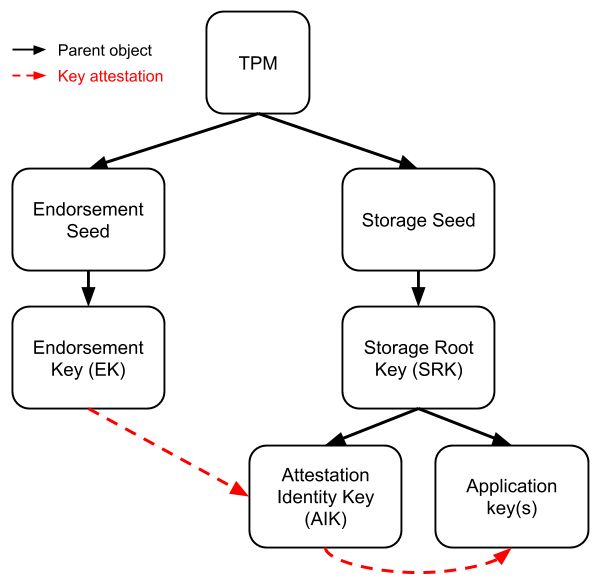
\includegraphics[width=0.55\textwidth]{figures/gerarchia-seed.png}
    \caption{Gerarchie dai seed TPM.}
    \label{fig:gerarchie_seed_tpm}
\end{figure}

In TPM 1.2, l'autorizzazione (il processo mediante il quale il software dimostra al TPM di essere autorizzato a utilizzare un oggetto) funziona tramite accesso con password e valori PCR. Per utilizzare una chiave, il software dovrà dimostrare la conoscenza dell'hash della password come parte del comando. L’\textit{Owner} era l’entità che conosceva la password, ma non era previsto distinguere tra un \textit{admin}, un utente o un manutentore per esempio. Quando più utenti condividono una piattaforma, diventa difficile condividere chiavi e dati TPM. Avere lo stesso meccanismo di autenticazione rende difficile gestire tanti ruoli in maniera indipendente ed efficace.

Dal TPM 2.0 i ruoli diventano concetti separati e previsti esplicitamente dalla specifica: esistono diverse autorizzazioni e \textit{policies} da combinare assieme, le responsabilità vengono distribuite su più gerarchie. Oltre alle due già citate (corrispondenti a \textit{endorsement seed} e \textit{storage seed}) la nuova specifica 2.0 prevede due gerarchie aggiuntive:
\begin{itemize}
    \item \textbf{Endorsement Hierarchy, \textbf{EH} (\textit{Endorsement Hierarchy}).} Utilizzata per tutte le operazioni sensibili alla privacy, autenticazione e per l'attestazione del dispositivo. Serve per generare certificati di identità e la chiave principale è la EK. Ogni dispositivo TPM ha un'unica EK che viene utilizzata per generare chiavi subordinate (AIK) per scopi di attestazione.
    \item \textbf{Storage Hierarchy, \textbf{SH} (\textit{Storage Hierarchy}).} Destinata all'uso del proprietario della piattaforma (azienda o l'utente finale). Utilizzata per operazioni non legate alla privacy, come la crittografia per proteggere i dati e la gestione delle chiavi di sessione. Praticamente replica la famiglia SRK della specifica precedente.
    \item \textbf{Platform Hierarchy, \textbf{PH} (\textit{Platform Hierarchy}).} Gerarchia definita dal produttore del chip, viene utilizzata per le funzioni di manutenzione e amministrazione. Le chiavi in questa gerarchia sono usate dagli aggiornamenti \textit{firmware}, \textbf{BIOS} (\textit{Basic Input/Output System}) etc. Non riguarda l’utente finale.
    \item \textbf{Null Hierarchy, \textbf{NH} (\textit{Null Hierarchy}).} Possiede il suo \textit{seed} unico, con chiavi primarie e derivate che però non possono essere preventive e persistenti. Il \textit{seed} è rigenerato a ogni reset del TPM: queste chiavi sono sempre effimere. 
\end{itemize}

L'Enhanced Authorization espande notevolmente i metodi con cui l'uso di chiavi e dati può essere autorizzato. In TPM 1.2, prima di ogni comando TPM ne veniva inviato un altro, che richiedeva l'autorizzazione per avviare la sessione: uno dei parametri del comando era un codice di autenticazione del messaggio, un hash della password che proteggeva l’accesso al comando stesso.

La EA estende queste sessioni di autorizzazione in \textit{policy sessions}, che permettono di combinare più metodi di autorizzazione (o politiche di autorizzazione) tramite logica booleana, creando di fatto un linguaggio di politica flessibile.  

Dal punto di vista operativo, la politica di sessione viene creata a livello software e poi associata ad un hash. Quando un comando TPM necessita di una certa politica, diventa sufficiente specificare l’hash ed il TPM avvierà una sessione di autorizzazione e invierà un comando dedicato per ogni \textit{token} di autorizzazione. Il TPM verificherà se l’hash della sequenza di comandi (con relativi input) sia lo stesso dell'hash della politica specificato al momento della creazione.

Per completezza, si sottolinea che non solo viene elaborato il nuovo meccanismo di politiche di autorizzazione, ma si prevedono nuovi metodi di autenticazione. Alcuni di questi sono: chiave HMAC del software, firma digitale, firma con dati aggiuntivi (forniti ad esempio da un lettore biometrico di impronte), indice della NVRAM o località di origine del comando.

\subsubsection{Quick key loading}
Nel TPM 1.2, la prima volta che una chiave veniva caricata, era necessario un processo di decodifica della chiave privata mediante l'uso della chiave privata del genitore della chiave stessa. Tale operazione risultava relativamente lenta. Per evitare la necessità di ripetere questa decodifica più volte durante una sessione, il TPM memorizzava temporaneamente la chiave decodificata nella sua \textit{cache}. Poiché si trattava di chiavi composte da una parte pubblica e una privata, l'esposizione della chiave pubblica non comportava rischi di compromissione. Sebbene il processo non utilizzasse crittografia simmetrica, questa soluzione consentiva al TPM di mantenere la chiave "pronta all'uso" durante l'intero ciclo di alimentazione, garantendo un accesso più rapido alla chiave nelle operazioni successive.

Durante il singolo ciclo di alimentazione, il TPM poteva ricaricare la chiave più velocemente rispetto alla ripetuta decodifica con la chiave privata del genitore. Tuttavia, al termine della sessione, e quindi con lo spegnimento, la chiave veniva cancellata e alla successiva accensione era necessario ripetere il processo di decodifica.

Con TPM 2.0, invece, a meno che una chiave non venga importata dall'esterno nel TPM, le chiavi memorizzate utilizzando memoria esterna sono cifrate con una chiave simmetrica. Questo approccio consente un caricamento rapido delle chiavi, eliminando la necessità di utilizzare una \textit{cache} per spostarle, a meno che non sia necessario l'accesso a una chiave genitore. Poiché il processo di decodifica è tanto veloce quanto il recupero di una chiave dalla \textit{cache}, non c'è motivo di usarla. Questo miglioramento permette un caricamento delle chiavi più efficiente, consentendo a più utenti di utilizzare un TPM senza riscontrare ritardi significativi. Di conseguenza, diventa più semplice progettare sistemi in cui più applicazioni possano accedere a un TPM in modo apparentemente illimitato.

\subsubsection{Non-brittle PCRs}
Nei primi modelli di TPM, in particolare nella versione 1.0, una delle principali problematiche era la fragilità dei valori PCR. I PCR registrano lo stato della macchina in diversi momenti del processo di avvio: i numeri più bassi rappresentano le prime fasi del \textit{boot}, mentre quelli più alti riflettono eventi successivi, fino all'avvio del sistema operativo. Per garantire maggior sicurezza, è possibile vincolare l'accesso a determinate chiavi e dati a specifici valori PCR, un meccanismo noto come \textit{sealing}. Tuttavia, questo approccio presentava alcune criticità, in particolare durante gli aggiornamenti del BIOS: se un segreto era bloccato a un valore PCR dipendente dal BIOS, un aggiornamento lo avrebbe reso inaccessibile, costringendo a sbloccarlo prima dell'operazione e a riassociarlo successivamente.

La specifica TPM 2.0 introduce un sistema più flessibile che consente di vincolare l’accesso alle risorse non a un valore PCR fisso, ma a una firma digitale rilasciata da un’entità di fiducia. Questo permette di recuperare i dati in più configurazioni approvate, ad esempio in base a versioni del BIOS validate da un'organizzazione IT o dal produttore dell’hardware. In questo modo, le risorse non sono più bloccate rigidamente a un singolo stato del sistema, ma possono essere recuperate in più configurazioni approvate.

I PCR permettono di bloccare alcuni valori tramite “\textit{sealing}”. Ma se questi valori sono chiavi o dati che rappresentano il BIOS, potrebbero presentarsi problemi qualora un valore serva prima dell’avvio del BIOS, prima fra tutte la casistica di \textit{update} al BIOS! Questa complicazione si chiama fragilità del PCR (o \textit{brittle PCR}). Questa maggiore flessibilità è resa possibile dal comando \texttt{TPM2\_PolicyAuthorize}, che permette di definire criteri di accesso dinamici (sulla base di EA). 

\subsubsection{Flexible Management}
La specifica 1.0 prevedeva due soli tipi di autorizzazione: quella della SRK e la \textit{owner authorization}. Spesso la SRK era settata a 20 bit tutti nulli ed utilizzata per molteplici scopi, rendendo difficile la gestione indipendente di tanti ruoli. La famiglia TPM 1.2 permetteva la delega, ma era complicata e raramente usata.

In TPM 2.0 vengono analizzati i diversi casi in cui l’autorizzazione tramite SRK veniva utilizzata e da questi sono ricavati diverse gerarchie di chiavi. Le gerarchie sono pensate per occuparsi di autorizzazioni e \textit{policy} diverse, rendendo la gestione di chiavi (e utenti) più leggera. Una descrizione più dettagliata delle gerarchie è stata fornita nella sezione 3.5.1.2.1 Le gerarchie.

\subsubsection{Identifying resources}
Nella specifica TPM 1.2, le risorse venivano identificate tramite un \textit{handle} anziché un nome legato alla risorsa stessa. Questo approccio apriva alla possibilità che un software di basso livello potesse modificare l'\textit{handle} identificativo, rendendo possibile indurre l’utente ad autorizzare un'azione diversa da quella che pensava di approvare. In tal modo, si creava una vulnerabilità che permetteva la manipolazione delle autorizzazioni.

Con l'introduzione del TPM 2.0, le risorse vengono ora identificate tramite un nome, che è vincolato alla risorsa, eliminando di fatto la vulnerabilità descritta. Inoltre, diventa possibile utilizzare una chiave TPM per firmare questo nome, garantendo così la sua correttezza. Il nome viene composto in modo da comprendere la \textit{policy} di autorizzazione della chiave, quindi firmare il nome equivale a firmare e validare le modalità attraverso cui è possibile autorizzare l'uso di una chiave. Questa firma funge anche da prova dell'integrità e dell'affidabilità della chiave, come descritto nel capitolo sull’EA. Se la chiave viene duplicata, la firma può fornire un "certificato di nascita", dimostrando quale TPM è stato utilizzato per la sua creazione.

\section{Variazioni del TPM 2.0}
Dalla specifica 2.0, il TPM diventa sempre più facile da implementare su diverse piattaforme, da PC a server a \textbf{SoC} (\textit{System on Chip}). Esistono quattro tipi principali di “forma di TPM” al momento, ognuna con i suoi pro e contro. In base al livello di sicurezza richiesto da un ambito è doveroso fare una valutazione dei costi e dei rischi per selezionare la forma che meglio si presta all’utilizzo specifico.

\subsection{Discrete TPM}
La forma del \textit{discrete} TPM (dTPM) è pensata per gli ambiti di sicurezza più alta e mira a rendere il dispositivo inviolabile, anche contro attacchi sofisticati. Per garantire questa protezione, il chip viene progettato e testato secondo standard rigorosi, resistendo a manomissioni avanzate come il \textit{probing} o il congelamento.

Si tratta di un modulo hardware fisicamente isolato e autonomo, integrato come un chip dedicato e collegato alla \textbf{CPU} (\textit{Central Processing Unit}) tramite un'interfaccia sicura. Le interfacce più comuni sono LPC (Low Pin Count), \textbf{I2C} (\textit{Inter-Integrated Circuit}), \textbf{SPI} (\textit{Serial Peripheral Interface}) e, occasionalmente, \textbf{PCIe} (\textit{Peripheral Component Interconnect Express}). L’uso di un collegamento dedicato riduce i rischi legati a interfacce condivise, limitando l’esposizione ad attacchi di intercettazione del \textit{bus} di comunicazione.

Il dTPM è adatto a proteggere sistemi critici, come nel controllo dei freni di un'automobile o di valvole in impianti che trattano materiali pericolosi. 

\subsection{Integrated TPM}
L'Integrated TPM (iTPM) rappresenta un livello di sicurezza inferiore rispetto al TPM discreto. Pur essendo una soluzione hardware, è integrato in un chip che svolge anche altre funzioni (come la CPU o il chipset). Risulta meno resistente alle manomissioni perché non possiede un’area isolata. Tuttavia, grazie alla sua implementazione hardware, mantiene una certa protezione contro le vulnerabilità \textit{software}. Questa soluzione offre un compromesso tra costi, prestazioni e sicurezza, perché mantiene comunque un buon livello di risorse di sicurezza dedicate.

\subsection{Firmware TPM}
Il \textit{firmware} TPM (fTPM) è una soluzione implementata tramite \textit{software} protetto, eseguibile direttamente sulla CPU principale senza la necessità di un chip separato. Il codice opera all'interno di un ambiente di esecuzione protetto, noto come \textbf{TEE} (\textit{Trusted Execution Environment}), che lo isola dagli altri programmi in esecuzione sulla CPU. In questo modo, informazioni sensibili come chiavi private, possono essere conservate nel TEE, rendendo più complesso l’accesso per eventuali attaccanti.

A differenza di un TPM hardware, l'fTPM non offre resistenza fisica alle manomissioni e la sua sicurezza dipende da diversi fattori, tra cui il sistema operativo del TEE e la presenza di vulnerabilità nel codice delle applicazioni eseguite al suo interno. Gli fTPM sfruttano il processore del sistema ospitante per creare un perimetro logico sicuro, basandosi su tecnologie hardware come \textbf{ARM} (\textit{Advanced RISC Machine}) TrustZone, Intel \textbf{SGX} (\textit{Software Guard Extensions}) e Intel Management Engine.

Dunque gli fTPM dipendono fortemente dalla capacità della CPU della piattaforma \textit{host} nel fornire un ambiente sicuro. Tuttavia se l’implementazione viene realizzata e progettata con le dovute accortezze, può garantire un buon livello di sicurezza.

\subsection{Software TPM}
Il \textit{Software} TPM (sTPM) è una soluzione implementata come un emulatore \textit{software} del TPM. Tuttavia, questa tipologia di TPM presenta numerose vulnerabilità, sia come possibilità di manomissione sia a causa della forte dipendenza da eventuali \textit{bug} nel sistema operativo su cui viene eseguita.

Gli sTPM non offrono protezione contro attacchi fisici o informatici e non sono considerati affidabili per applicazioni che richiedono un elevato livello di sicurezza. Un aspetto interessante è il loro utilizzo anche in ambienti \textit{cloud}, dove vengono implementati a livello di \textit{hypervisor} per la gestione della sicurezza virtualizzata.

Nonostante le sue limitazioni in termini di sicurezza, l’sTPM ha applicazioni specifiche, risultando particolarmente utile per attività di test o per la progettazione di prototipi di sistemi che prevedono l’integrazione di un TPM senza la possibilità di operare direttamente su un chip. In questi contesti, può rappresentare una soluzione adeguata per la sperimentazione e la validazione del \textit{software}.

\subsection{Virtual TPM}
Molti sistemi \textbf{IoT} (\textit{Internet of Things}) includono sensori e elaborazione \textit{cloud}, il che implica l’impiego di tecniche di virtualizzazione. L'uso delle macchine virtuali (\textbf{VM} [\textit{Virtual Machine}]) sicuramente offre flessibilità nell'elaborazione dei dati, ma aumenta sensibilmente anche il rischio di attacchi a causa della sua natura virtuale.

L'integrazione di un Virtual TPM (vTPM) consente di verificare l'assenza di attività malevole prima dell'avvio del processo di \textit{boot} di una macchina virtuale, rafforzando così la sicurezza del sistema. 

In un ambiente \textit{cloud}, il vTPM si inserisce come una soluzione intelligente per la protezione, in quanto fa parte dell'infrastruttura basata su \textit{cloud} e distribuisce i comandi a ciascuna macchina virtuale separatamente. A differenza di un TPM tradizionale, che si concentra sulla protezione del dispositivo \textit{host}, il vTPM è progettato per proteggere gli ambienti virtualizzati, dove più macchine virtuali, ognuna con il proprio sistema operativo, possono essere eseguite su un singolo \textit{host}. 

Il vTPM emula le funzionalità di archiviazione sicura di un TPM hardware e compie operazioni crittografiche direttamente nel \textit{software}, offrendo gli stessi comandi di un TPM fisico. Consente al sistema operativo \textit{guest} di generare e conservare chiavi private, migliorando così le misure di sicurezza disponibili. Le chiavi vengono isolate dal sistema principale, riducendo il rischio di compromissione durante eventuali attacchi. Il vTPM riceve informazioni crittografiche da un'autorità di certificazione (CA), simile alla chiave di crittografia (EK) di un TPM fisico, e le chiavi generate vengono utilizzate esclusivamente dal sistema operativo per operazioni di crittografia e firma digitale. Ciò consente la validazione remota dell'identità e dell'affidabilità della macchina virtuale, così come la verifica del \textit{software} in esecuzione.

Tuttavia, nonostante i vantaggi, i vTPM presentano alcune vulnerabilità. Poiché sono implementati tramite \textit{software}, sono soggetti ad attacchi legati alle debolezze del sistema operativo sottostante e della virtualizzazione stessa. L'isolamento offerto dal vTPM dipende fortemente dalla sicurezza dell'infrastruttura di virtualizzazione. Inoltre, i vTPM non offrono la stessa resistenza fisica alle manomissioni dei TPM hardware, il che li rende più suscettibili ad attacchi mirati.